% !TeX spellcheck = pl_PL 
\chapter{Analiza tematu}
\section{Podstawowe pojęcia}
\subsection{Definicja grafu}\label{ssec:graphDef}
\textit{Sieć przepływowa} $ G=(V, E) $ jest grafem prostym skierowanym; strukturą, która składa się z dwóch zbiorów:
\begin{itemize}
	\item \textit{n}-elementowego zbioru wierzchołków $ V = \{v_1,v_2,...,v_n \}$
	\item \textit{m}-elementowwgo zbioru uporządkowanych łuków $ E = \{e_1,e_2,...,e_m \}$, gdzie $ e_i=(v_j,v_k);\quad i=1,...,m;\quad v_j,v_k\in V$. Innymi słowy, każdy łuk jest parą wierzchołków należących do zbioru $ V $.
\end{itemize}
\textit{Grafem prostym} nazywany taki graf w którym nie istnieją \textit{pętle}. Pętlą nazywamy łuk $ (v_j,v_k) $ dla którego $ v_j=v_k $. W sieci przepływowej wyróżnia się dwa wierzchołki: źródło $ s \in V $ oraz ujście $ t \in V $. W sieci przepływowej definiuje się ponadto \textit{funkcję przepustowości} $ c : E\rightarrow R_{\ge0}$ odwzorowującą zbiór łuków w zbiór liczb rzeczywistych. Dodatkowo, w celu uproszczenia dziedziny, zakłada się, że z każdego wierzchołka u $ v\in V\backslash\{s, t\} $ istnieje ścieżka prowadząca ze źródła do ujścia. Założenie to ma zapewnić, że w rozpatrywanych grafach będzie istniała co najmniej jedna ścieżka ze źródła do ujścia.\\\indent
\textit{Przepływ} w sieci $ G $ jest funkcją $ f $, która odwzorowuje zbiór łuków w zbiór liczb rzeczywistych $ f : E \rightarrow R_{\ge0} $ i spełnia następujące założenia:
\begin{itemize}
	\item Warunek przepustowości: $ \forall_{v_i, v_j\in V} : f(v_i, v_j) \le c(v_i, v_j) $.\\Przepływ w żadnym z łuków nie może przekroczyć jego przepustowości.
	\item Warunek skośnej symetryczności: $ \forall_{v_i, v_j\in V} : f(v_i, v_j) = -f(v_j, v_i) $.\\Przepływ w przeciwnym kierunku traktujemy jakby posiadał wartość ujemną.
	\item Warunek zachowania przepływu: $ \forall_{v\in V\backslash\{s, t\}} : \sum_{u\in V}f(v,u)=\sum_{u\in V}f(u,v) $.\\Suma przepływów wpływających do wierzchołka musi być równa sumie przepływów wypływających z niego.
\end{itemize}
\subsection{Przepływ netto}\label{ssec:netto}
Przepływem netto nazywamy wartość funkcji przepływu $ f(v_i, v_j) $ pomiędzy wierzchołkami $ v_i $ oraz $ v_j $. Zgodnie z warunkiem skośnej symetryczności, wartość może być dodatnia lub ujemna. Dodatnia oznacza przepływ z wierzchołka $ v_i $ do wierzchołka $ v_j $, natomiast ujemna - w przeciwnym kierunku. Sieć przepływowa jest grafem skierowanym, więc dla dwóch wierzchołków może posiadać parę sąsiednich łuków. Poniższy przykład przedstawia istotę przepływu netto, jeżeli w obu sąsiadach istnieje niezerowy przepływ.
\begin{figure}[h]
	\centering
	\begin{subfigure}{0.25\textwidth}
		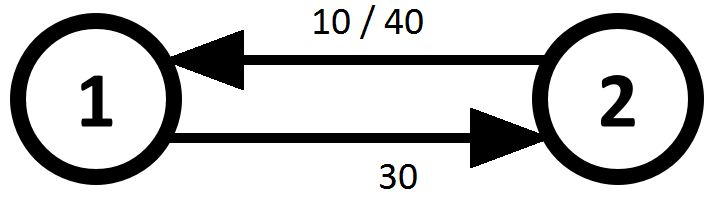
\includegraphics[width=0.9\linewidth]{./img/netto1.png} 
		\caption{}
		\label{fig:netto1}
	\end{subfigure}
	\begin{subfigure}{0.25\textwidth}
		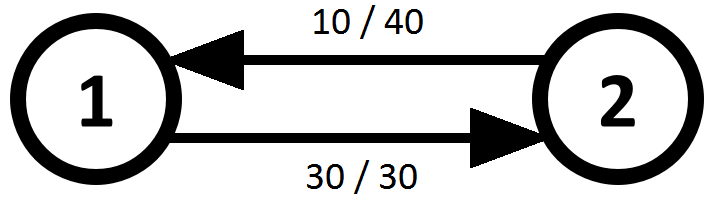
\includegraphics[width=0.9\linewidth]{./img/netto2.png}
		\caption{}
		\label{fig:netto2}
	\end{subfigure}
	\begin{subfigure}{0.25\textwidth}
		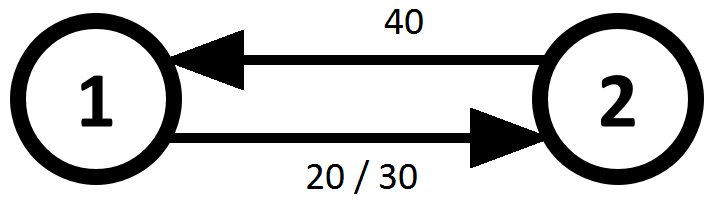
\includegraphics[width=0.9\linewidth]{./img/netto3.png}
		\caption{}
		\label{fig:netto3}
	\end{subfigure}
	\caption{Zobrazowanie przepływu netto}
	\label{fig:imageNetto}
\end{figure}\vfill
Na rysunku \ref{fig:netto1} istnieje przepływ z wierzchołka 2 do wierzchołka 1 o wartości 10, czyli $ f(2, 1) = 10 $. Zgodnie z warunkiem skośnej symetryczności $ f(1, 2) = f(2, 1) = -10 $. Można powiedzieć, że wierzchołek 2 opuszcza 10 jednostek materiału, które wpływają do wierzchołka 1. Na rysunku \ref{fig:netto2} pojawia się drugi przepływ, z wierzchołka 1 do wierzchołka 2 przepływa 30 jednostek. W tym przypadku wartość przepływu w istocie jest równa $ f(1,2)=-10 + 30=20 $. Jest to równoznaczne sytuacji, w której istnieje tylko przepływ 20 jednostek z wierzchołka 1 do wierzchołka 2. Przepływ z wierzchołka 2 do wierzchołka 1 zostaje zmniejszony do $ f(2, 1)=10-30=-20 $, co jest zgodne z warunkiem zachowania skośności.
\subsection{Maksymalny przepływ w sieci}
Wartość przepływu $ |f| $ w sieci jest definiowana jako suma przepływów netto wychodzących ze źródła $ \sum_{v\in V}{f(s, v)} $. Zgodnie z warunkiem zachowania przepływu, jest ona równa sumie wartości przepływów netto wpływających do ujścia $ \sum_{v\in V}{f(v, t)} $. Problem maksymalnego przepływu polega na znalezieniu maksymalnej wartości $ |f| $ w sieci przepływowej.\cite{id:ZaawansowaneAlgorytmyStruktury}
\subsection{Sieć residualna}
\section{Algorytmy znajdowania maksymalnego przepływu}
\section{Wykorzystane technologie}